---
id: tkz-euclide-ejemplo-57
title: "Triángulo escaleno"
description: "Creación de un triángulo escaleno"
keywords: [angulo,triangulo,escaleno,taller2]
tags: [tkzDefTriangle,tkzMarkSegment,tkzMarkAngle,tkzFillAngle,tkzDrawPolygon]
sort: 57
---
\documentclass[tikz,border=2mm]{standalone}
\usepackage{xcolor}
\usepackage{tkz-base}
\usepackage{tkz-euclide}

\begin{document}
    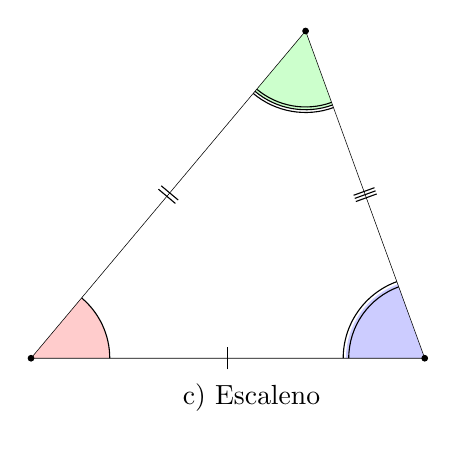
\begin{tikzpicture}
        % Paso 1: Define los puntos de la base GH
        \tkzDefPoint(12,1){G}
        \tkzDefPoint(17,1){H}

        % Paso 2: Define triangulo escaleno △GHI 
        % (con ángulos 50°, 70°, 60°), recupera punto I
        \tkzDefTriangle[two angles = 50 and 70](G,H)
            \tkzGetPoint{I}

        % Paso 3: Marca y rellena ángulos congruentes
        \tkzFillAngle[fill=red!20](H,G,I)
        \tkzFillAngle[fill=blue!20](I,H,G)
        \tkzFillAngle[fill=green!20](G,I,H)        

        % Paso 4: Dibuja los puntos y el polígono
        \tkzDrawPoints(G,H,I)
        \tkzDrawPolygon(G,H,I)

        % Paso 5: Marca los segmentos
        \tkzMarkSegment[mark=|](H,G)
        \tkzMarkSegment[mark=||](G,I)
        \tkzMarkSegment[mark=|||](H,I)        
        
        % Paso 6: Marca los angulos
        \tkzMarkAngle[arc=l](H,G,I)
        \tkzMarkAngle[arc=ll](I,H,G)
        \tkzMarkAngle[arc=lll](G,I,H)

        % Paso 7: Agrega una leyenda al gráfico
        \tkzText(14.8,0.5){c) Escaleno}
    \end{tikzpicture}
\end{document}